\documentclass[10pt,a4paper]{article}
\usepackage[utf8]{inputenc}
\usepackage{amsmath}
\usepackage{amsfonts}
\usepackage{amssymb, graphicx}
\usepackage[left=2cm,right=2cm,top=2cm,bottom=2cm]{geometry}
\graphicspath{{../figures/}}
\author{Susanna Makela}
\title{Exploring Centered vs Non-centered Parameterizations in Stan}
\begin{document}
\maketitle

\section*{Introduction}
In running simulations with a simple hierarchical model, I noticed that the centered parameterization often outperformed the non-centered one. I thought that was strange, since from what I've read (cite things here), it seems like the non-centered parameterization would be superior in most cases. To get a better idea of what's going on, I did a quick simulation using a simple model with varying intercepts:
\begin{align*}
	y_i &\sim N(\beta_{0j[i]} + \beta_1 x_i, \sigma_y^2), \quad \text{for } i = 1, \ldots, N \\[3pt]
	\beta_{0j} &\sim N(\mu_0 + \gamma_0 w_j, \tau_0), \quad \quad \text{for } j = 1, \ldots, J,
\end{align*}
where the notation $j[i]$ indicates the group $j$ to which unit $i$ belongs. Here $x_i$ is a unit-level predictor and $w_j$ is a group-level predictor.

\section*{Models}
To see how the presence of these predictors affects the efficiency of each parameterization, I created several variations on the above model as described below.

\begin{enumerate}
	\item No unit- or group-level predictors; $\beta_1 = 0, \gamma_0 = 0$ \\[4pt]
	$\begin{aligned}[t]
	  y_i &\sim N(\beta_{0j[i]}, \sigma_y^2) \\[3pt]
	  \beta_{0j} &\sim N(\mu_0, \tau_0) \\[3pt]
	\end{aligned}$
	\item Group-level predictor only; $\beta_1 = 0$ \\[4pt]
	$\begin{aligned}[t]
	  y_i &\sim N(\beta_{0j[i]}, \sigma_y^2) \\[3pt]
	  \beta_{0j} &\sim N(\mu_0 + \gamma_0 w_j, \tau_0) \\[3pt]
	\end{aligned}$
	\item Unit-level predictor only; $\gamma_0 = 0$ \\[4pt]
	$\begin{aligned}[t]
	  y_i &\sim N(\beta_{0j[i]} + \beta_1 x_i, \sigma_y^2) \\[3pt]
	  \beta_{0j} &\sim N(\mu_0, \tau_0) \\[3pt]
	\end{aligned}$
	\item ``Full'' model \\[4pt]
	$\begin{aligned}[t]
	  y_i &\sim N(\beta_{0j[i]} + \beta_1 x_i, \sigma_y^2) \\[3pt]
	  \beta_{0j} &\sim N(\mu_0 + \gamma_0 w_j, \tau_0) \\[3pt]
	\end{aligned}$
\end{enumerate}
I generated data from each model for three values of $J$ and five values of $\tau_0$:
\[
	J = 5, 15, 30, \quad \text{and} \quad \tau_0 = 0.001, 0.01, 0.1, 1.0, 10.
\]
I set $\beta_1 = 0.5$ and $\gamma_0 = 0.8$ (except as described above), $\mu_0 = 0.2$, $\sigma_y = 0.05$, and  sampled 30 values of $y_i$ in each group, so that $N = 30J$. I created the predictors $x_i$ as $x_i \sim U(-1, 1), ~i = 1, \ldots, N$ and $w_j$ as $w_j \sim U(-1, 1), ~j = 1, \ldots , J$. I used the same seed for generating each dataset, so they have varying amounts of overlap.

\section*{Stan models}
For each simulated dataset, I fit the corresponding model from which it was generated. I added the weakly informative priors,
\begin{align*}
	\pi(\mu_0) &\sim N(0, 1) \\
	\pi(\gamma_0) &\sim N(0, 1) \\
	\pi(\tau_0) &\sim \text{Half-Cauchy}(0, 2.5) \\
	\pi(\beta_1) &\sim N(0, 1) \\
	\pi(\sigma_y) &\sim \text{Half-Cauchy}(0, 2.5),
\end{align*}
omitting the priors for $\gamma_0$ and $\mu_0$ in models 1-3 as appropriate. Each time, I ran Stan for 2,000 iterations with four chains and the parameter \texttt{adapt\_delta} set to 0.99. Note that there were some instances where Stan returned warnings about divergent transitions.

\section*{Results}
Figure \ref{fig:results} shows the results of fitting each of the four models described above to data generated from that model, using both the centered and non-centered parameterizations. The $y$-axis is the effective sample size (ESS) per second for $\tau_0$, the group-level standard deviation of the random intercepts, against the true value of $\tau_0$ under which the data were generated. The columns correspond to the four models and the rows to the number of groups $J$ in the data.

Surprisingly, in contrast to the results of Betancourt and Girolami (though that was slightly different model), the centered parameterization always performs better for $\tau_0 > 0.1$. When the number of groups is small ($J = 5$), the non-centered parameterization is better only when the group-level variance is very small ($\tau_0 = 0.001$) and the model includes both a unit- and a group-level predictor.

\begin{figure}[h!]
	\begin{center}
		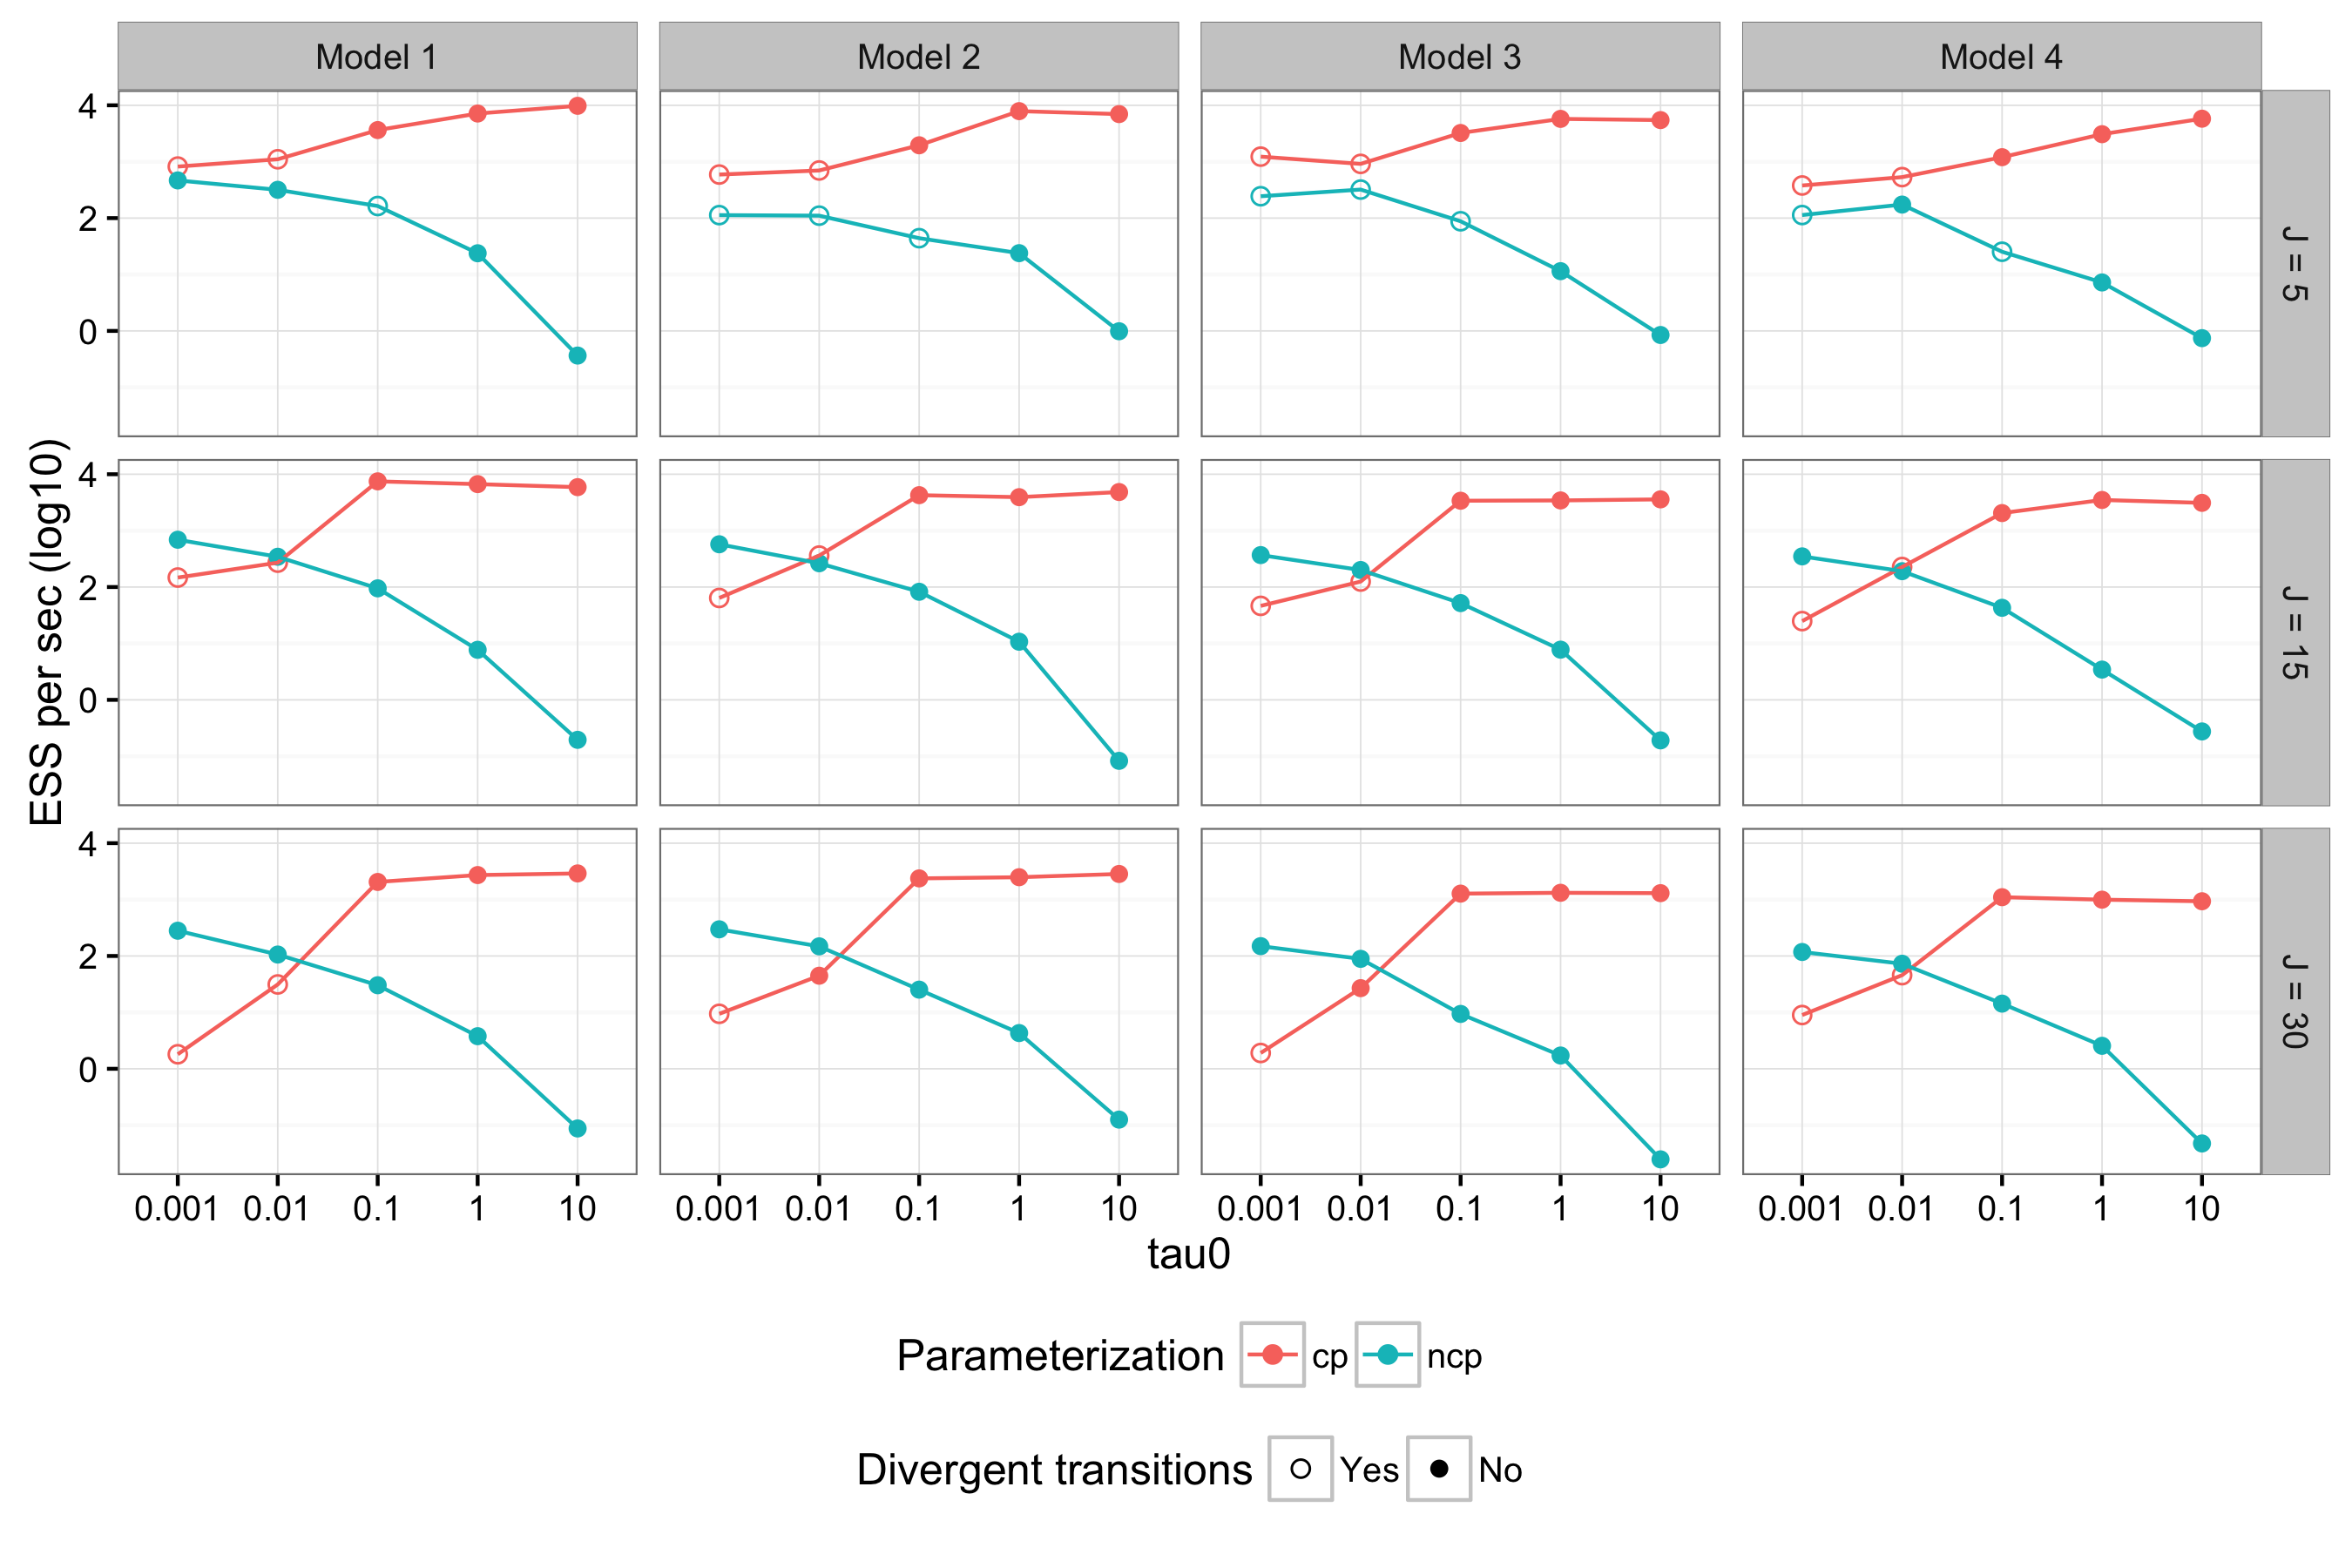
\includegraphics[scale=0.175]{tau0_ess_per_sec.png}
		\caption{Plots of effective sample size (ESS) per second ($\log_{10}$ scale) against $\tau_0$, the group-level variability of the random intercepts. The rows are for the number of groups $J$, and the columns are for the four models described in Models. cp = centered parameterization; ncp = non-centered parameterization.}
		\label{fig:results}
	\end{center}
\end{figure}




\end{document}